\subsection{Evaluación de modelo}  
    Luego de construir un modelo, es importante poder determinar qué tan bueno es para predecir la variable dependiente. La manera de hacer esto es, después de entrenar nuestro modelo, comparar los resultados obtenidos con los datos reales.
    
    %decir que tan bueno es, se debe observar su capacidad de estimar la variable dependiente ( la que se quiere predecir ) en base a valores de las variables independientes ( predictores ) y comparar el error de la estimación con respecto al valor real de la variable dependiente.
    
    \subsubsection{Métricas}
  
    Para realizar estas comparaciones, una primera idea suele ser medir el promedio de las diferencias absolutas entre los datos reales, y nuestras predicciones. El problema con esta idea es que hay casos donde esta métrica puede verse afectada según la naturaleza de la variable que se intenta predecir. En pos de solucionar los problemas que pueda tener una métrica en particular, lo que se hace es tener en cuenta un conjunto de ellas, con la intención de obtener los modelos con los mejores resultados en conjunto. A continuación, exponemos las métricas que usamos en nuestra experimentación.
    
    %Para poder llevar a cabo esta comparación, hay varias métricas que la resuelven, de las cuales mencionamos las tres que consideramos para nuestro análisis.

        \paragraph{RMSE (Root Mean Squared Error)}\mbox{}\vspace{1em}
        
        Una métrica un poco más avanzada que el promedio de las diferencias absolutas, y en sintonía con el método de cuadrados mínimos, es la que se conoce como \emph{RMSE} (root mean squared error), que consiste en calcular la raíz cuadrada del promedio de los errores cuadráticos entre las predicciones y los datos. Formalmente, la métrica está definida de la siguiente manera:
        %Una primera idea para calcular el error cometido en la predicción es la del RMSE ( Root Mean Squared Error ), que equivale a hacer:
        
        \[ RMSE= \sqrt{\frac{1}{n}\sum_{j=1}^{n} (f(X_j) - Y_j)^2}\]
        
        Donde $X_j$ la muestra $j$-esima, $f$ es la función del modelo, y $Y_j$ es el valor real a predecir para cada muestra.
        
        Esta métrica busca representar al error cometido al estimar como el promedio de los errores cometidos para cada valor de la variable dependiente $y$. Esta métrica resulta intuitiva y razonable, porque es  lo que se puede pensar en hacer en una primera instancia, pero presenta un problema grave.
        
        %Esta métrica busca , a grandes rasgos, representar al error cometido al estimar como el promedio de los errores cometidos para cada valor de la variable dependiente $y$. Esta métrica resulta intuitiva y razonable, porque es lo que se puede pensar en hacer en una primera instancia, pero presenta un problema grave.
        
        El defecto del \emph{RMSE} es que, cuando se comete un error grande para cierto valor de $y$, eso repercute mucho en el promedio de los errores. Es decir, si había un valor a estimar que era grande comparado con otros valores que tomaba la variable $y$, este va a tener mayor peso en el error que otros.
        
        \paragraph{RMSLE (Root Mean Logarithm Squared Error)}\mbox{}\vspace{1em}
        
        Existe una segunda métrica casi idéntica a la anterior, que introduce al calculo de \emph{RMSE} una solución al problema que tiene el mismo. Podemos ver a continuación la nueva definición del error:
        
        \[ RMSLE= \sqrt{\frac{1}{n}\sum_{j=1}^{n} (\log{(f(X_j))} - \log{(Y_j)})^2}\]
        
        Donde $X_j$, $f$ e $Y_j$ son las mismas que en \emph{RMSE}.
        
        Lo que cambia en este caso, es que ahora no se calcula la diferencia directamente, sino que primero se aplica el logaritmo a ambos términos, tanto $f(x)$ como $y$, antes de realizar la diferencia entre ellos.
        
        La idea atrás de esto es que, si bien RMSE tiene sentido, tiene problemas al tratar con variables que presentan valores grandes, como son los outliers. Entonces, como solución, se le aplica el logaritmo a estas variables, para luego poder trabajar con números mas pequeños, y que todos aporten equitativamente al calculo del error.
        
        
        \paragraph{$\mathbf{R^2}$ (R-squared)}\mbox{}\vspace{1em}
        
        Además de interesarnos por medir el error de un modelo, nos interesó también poder capturar si había espacio para mejorarlo. Para poder analizar esto, optamos por utilizar la métrica R2, la cual se muestra a continuación:
        
        \[ R2= 1 - \frac{\sum_{j=1}^{n} (f(X_j) - Y_j)^2}
                    {\sum_{j=1}^{n} (\overline{Y} - Y_j)^2}\]
        
        Donde $X_j$, $f$ e $Y_j$ son las mismas que en $RMSE$, y $\overline{Y}$ es la media de las muestras $Y_j$.
        
        Es importante notar que el resultado suele variar entre 0 y 1 , siendo 1 el resultado de un modelo que no puede mejorase, y por lo contrario, 0 el resultado si hubiéramos tomado el promedio. Sin embargo, en la práctica podría suceder que un modelo sea peor que el promedio, lo cual llevaría a un r2 negativo. Lo que refleja este calculo se puede ver mejor en este gráfico:
        
        \begin{figure}[H]
            \centering
            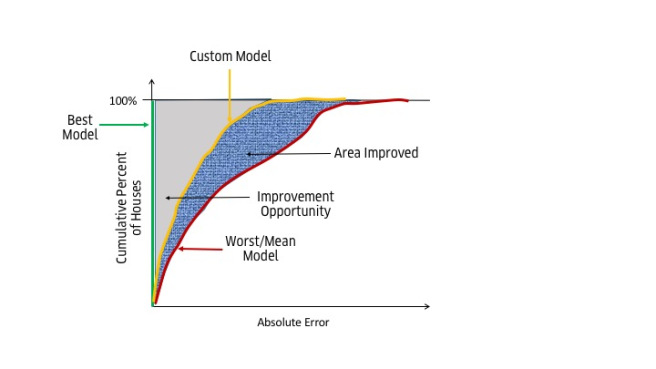
\includegraphics[scale=0.5]{img/explicaciones/R2-Curves.jpg}
            \caption{Resultado del \textit{Curvas de R2}}
            \label{fig:R2-Curves}
        \end{figure}
        
        En este se muestran 3 curvas, una por cada posible modelo.
        El \textbf{Best Model} es el mejor modelo teórico, donde el error acumulado siempre es 0. Luego se tiene el \textbf{Worst Model}, que representa a un regresor que solo tiene en cuenta el promedio de los datos.
        Finalmente, se tiene al \textbf{Custom Model}, el modelo que uno diseña, el cual tiene un error que se encuentra entre la del mejor y el peor modelo. También se puede observar que la manera de interpretar el gráfico es observando el área debajo de la curva de un modelo.
        Si observamos la curva del \textbf{Custom Model}, observamos que el área azul encerrada entre esta curva y la del \textbf{Worst Model} indica cuanto se mejoró con respecto a este último. Así también, el área gris, encerrada entre el \textbf{Custom Model} y el \textbf{Best Model}, indica cuanto puede mejorarse para parecerse a este ultimo modelo.
        
\subsubsection{K-Fold cross validation}

 %   determinar como se generalizan estos resultados en práctica. Teniendo simplemente dos conjuntos de datos, uno de entrenamiento, y otro de preba, a veces el modelo es suceptible a la distribución de los datos de entrenamiento. El objetivo del método de \cv es intentar aisalar al modelo, de problemas como  \emph{overfitting} o \emph{selection bias}, y mostrar como operaria el modelo con datos independiente. K fold cross validarion es dividir el dataset en $k$ particiones de igual tamaño.
    
    Al utilizar estas métricas para medir el error o la mejora de un modelo, se suele definir un conjunto de training y otro de validation. Luego, se hace un \textit{training} del modelo con el primer conjunto, y luego se aplica el \textit{predict} sobre el segundo conjunto. Y finalmente, se aplica alguna de las métricas sobre el resultado del \textit{predict}, y se obtiene el error cometido o si se mejoró o no el modelo.
    
    El problema de este procedimiento es que se esta definiendo un conjunto como training y otro como validation, y no se los cambia más. Esto provoca que al minimizar, por ejemplo, el error, bajo un mismo conjunto no necesariamente implica que en el caso general sea mejor, ya que no se está midiendo para distintos conjuntos de training y validation.
    
    Una forma de solucionar este problema es la de intentar evaluar bajo distintos conjuntos de training y validation y tomar el promedio de todos ellos. Para esto existe la técnica de \emph{K-Fold cross validation}, que busca solucionar el problema mencionado aplicando variaciones en los conjuntos para luego aplicar las métricas. Podemos ver esto mas claramente en el siguiente diagrama:
    
    \begin{figure}[H]
        \begin{center}
            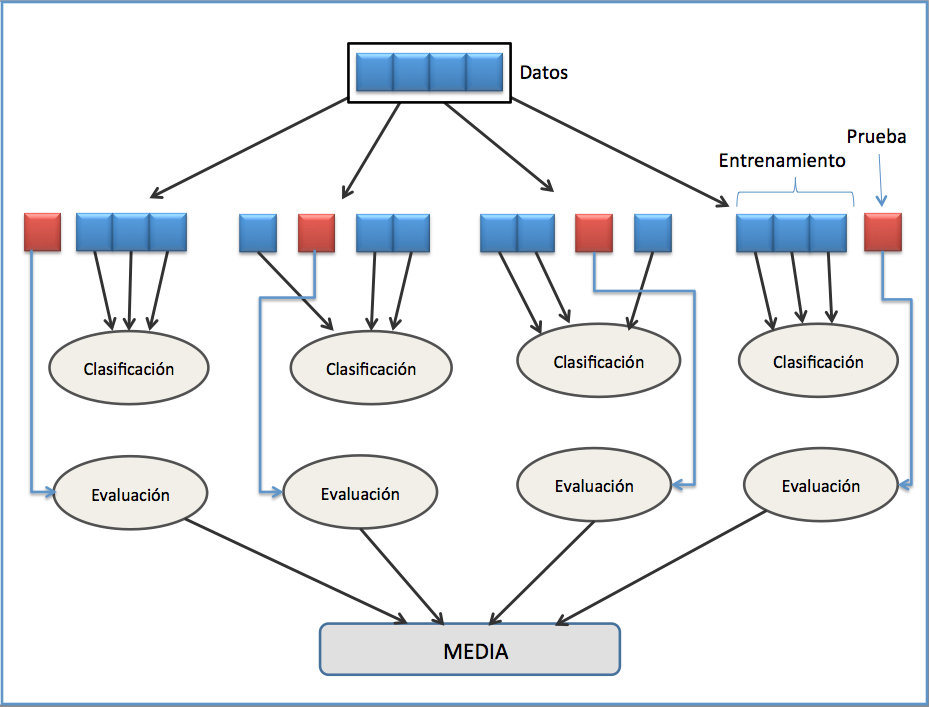
\includegraphics[scale=0.3]{img/explicaciones/k_fold.png}
        \end{center}
        \caption{Diagrama K-Fold}
    \end{figure}
    
    En este caso particular, se tiene un conjunto de datos que se lo divide en 4 conjuntos de igual tamaño. Luego, se toma en cada caso 3 conjuntos para training y el otro para validation. Con estos 2 nuevos conjuntos finales de training y de validation, se entrena al modelo y luego se lo evalúa, generando un resultado. Este proceso se repite para cada variación de conjunto de training y validation, y se obtiene la media de los resultados obtenidos. Esta media va a ser entonces la que se va a intentar maximizar bajo el criterio establecido.